% Created 2020-10-30 sex 14:16
% Intended LaTeX compiler: pdflatex
\documentclass[11pt]{article}
\usepackage[utf8]{inputenc}
\usepackage{lmodern}
\usepackage[T1]{fontenc}
\usepackage[top=3cm, bottom=2cm, left=3cm, right=2cm]{geometry}
\usepackage{graphicx}
\usepackage{longtable}
\usepackage{float}
\usepackage{wrapfig}
\usepackage{rotating}
\usepackage[normalem]{ulem}
\usepackage{amsmath}
\usepackage{textcomp}
\usepackage{marvosym}
\usepackage{wasysym}
\usepackage{amssymb}
\usepackage{amsmath}
\usepackage[theorems, skins]{tcolorbox}
\usepackage[style=abnt,noslsn,extrayear,uniquename=init,giveninits,justify,sccite,
scbib,repeattitles,doi=false,isbn=false,url=false,maxcitenames=2,
natbib=true,backend=biber]{biblatex}
\usepackage{url}
\usepackage[cache=false]{minted}
\usepackage[linktocpage,pdfstartview=FitH,colorlinks,
linkcolor=blue,anchorcolor=blue,
citecolor=blue,filecolor=blue,menucolor=blue,urlcolor=blue]{hyperref}
\usepackage{attachfile}
\usepackage{setspace}
\usepackage{tikz}
\addbibresource{refs.bib}
\usepackage{svg, caption, multirow, booktabs}
\usepackage[english]{babel}
\author{Gabriel Petrini, Lucas Teixeira}
\date{\today}
\title{Long-run effective demand and residential investment: a Sraffian supermultiplier based analysis}
\begin{document}

\maketitle
\begin{abstract}
In this paper, we build a fully specified parsimonious Sraffian supermultiplier stock-flow consistent model (SSM-SFC) with two non-capacity creating autonomous expenditure: residential investment and debt-financed consumption.
Our model represents a closed and without government economy with workers and capitalist households and only the latter are not not credit constrained.
The introduction of residential investment implies that our SSM-SFC model has two real assets: firms' productive capital and households' real estate.
The numerical simulation experiments report the main standard Sraffian supermultiplier growth models results: 
    (i) income distribution affects growth rate only during the traverse;
    (ii) autonomous expenditures alone affects long-term growth rate and;
    (iii)  utilization rate moves towards the normal one.
As a particular result, an increase of residential investment growth rate increase implies a decrease of real estate share in total real assets.
Therefore, this model introduces both housing and asset bubbles	on Sraffian supermultiplier agenda and extends the range of autonomous expenditures alternatives.

\noindent \textbf{Keywords:} Residential Investment; Sraffian supermultiplier; Asset bubble;  Stock-Flow Consistent approach.
\end{abstract}


\section{Introduction}
\label{sec:org6b4a813}
\label{sec:introduction}

Non-residential investment is the most scrutinized variable in demand-led growth models so that others expenditures play a secondary role \cite{brochier_macroeconomics_2017}.
A decade after the Great Recession, this is still the case for residential investment which continues to receive sparse and unsystematic attention by the literature \cites{caverzasi_stock-flow_2013}{nikolaidi_minsky_2017}.
Despite its absence in theoretical models, there is a growing empirical literature highlighting its macrodynamic relevance \cites{leamer_housing_2007}{jorda_great_2014}{fiebiger_semi-autonomous_2018}{fiebiger_trend_2017}.
In this paper, we try to fill this gap in demand-led growth agenda.


Sraffian supermultiplier growth model (SSM) establishes an important role to non-capacity creating (NCC) autonomous expenditures.
\textcite{serrano_long_1995} --- and also more recent papers \cite{freitas_growth_2015} --- presents the SSM model in a rather parsimonious way as an alternative closure within demand-led growth model agenda \cite{serrano_sraffian_2017}.
More recently, SSM has been introduced to a broader Post-Keynesian audience by \textcites{allain_tackling_2015}{lavoie_post-keynesian_2015}{lavoie_convergence_2016}.
In summary,  SSM describes a demand-led growth pattern led by NCC autonomous expenditures such as residential investment.


Different NCC autonomous expenditures have been included in this framework. 
For instance, some scholars have investigated the macroeconomic implications of both debt-financed \cites{pariboni_autonomous_2015}{fagundes_role_2017}{mandarino-2020-worker-debt} and financial wealth-financed consumption \cite{brochier_supermultiplier_2018}.
The same applies to government expenditures \cites{allain_tackling_2015}{bougrine_autonomous_2020} and exports \cite{nah_long-run_2017}.

\textbf{Nota:} Os dois parágrafos seguintes não estavam na versão anterior.

Even though these works emphasize the relevance of some NCC autonomous expenditures, residential investment has been systematically neglected.
To be fair, \textcites{zezza_u.s._2008}{nikolaidi_securitisation_2015} include residential investment in a SFC growth model.
However, as a result of neo-Kaleckian non-residential investment function specification, residential investment does not lead the business cycle and plays a secondary role.
In a recent contribution, \textcite{dejuan_supermultiplier-cum-finance_2018} presents an SSM model with residential investment in order to analyze household over-indebtedness.
In summary, we report an increasing attention to the macroeconomic implications of residential investment.
%However, there has been little discussion about the connection between housing bubble and aggregate demand.

Despite the importance of the recent housing bubble episode, little attention has been paid to the connection between asset bubbles and aggregate demand.
This paper attempts to fill this gap. 
One way to do this is through houses' own rate of interest proposed by \textcite{teixeira_crescimento_2015}.
Originally introduced by \textcite{Sraffa_Own_1932}, this concept DESCREVER TAXA PRÓPRIA.
In summary, this particular real interest rate is the relevant one for house investors (households). 

Based on this concept, this paper attempts to connect asset bubble and aggregate demand within a Sraffian Supermultiplier Stock-Flow Consistent framework. 
The remainder of this paper is organized as follows.
Section \ref{sec:empirical} introduces the so-called houses own rate of interest and some residential investment related stylized facts for the US economy.
%Section ref:sec:Review reviews heterodox growth models with NCC autonomous expenditures and highlights the lack of residential investment as an autonomous expenditure.
Section \ref{sec:Model} presents a SSM-SFC model  with asset bubbles and two real assets: firms' capital and household' real estate. 
Section \ref{sec:runs} evaluates short-run, traverse and fully-adjusted position equilibria in order to access the consequences of residential investment inclusion on stock-flow consistent ratios.
Next, in Section \ref{sec:Experiments}, both traverse and steady-state dynamics are evaluated through numerical simulations.
Inspired by the recent housing bubble episode, the experiments are: decrease in wage-share (Section \ref{sec:Exp1}); increase in real estate inflation (Section \ref{sec:Exp2}); and an increase in interest rate \ref{sec:Exp3}).
In this same Section, we also plug houses own rate of interest observed data for the U.S. (from 1992 to 2019) in order to compare simulations' results with the stylized facts presented previously.
Section \ref{sec:Conclusion} offers some concluding remarks while Appendix \ref{append:Solution} presents some partial derivatives and Appendix \ref{append:Data} provides simulation's parameters and baseline values.



\section{Empirical Motivation}
\label{sec:orgcec45fe}
\label{sec:empirical}

A current trend among empirical research on demand-led growth is about the role of NCC autonomous expenditures.
\textcite{freitas_pattern_2013} present a growth accounting decomposition and report the relevance of those expenditures in explaining Brazilian GDP growth between 1970 and 2005. \textcite{braga_investment_2018} shows evidence that economic growth and non-residential investment are explained by NCC autonomous expenditures in Brazilian economy from 1962 to 2015. For the U.S., \textcite{girardi_long-run_2016} show that NCC autonomous expenditures have permanent effects on growth rate. 
\textcite{haluska_growth_2019} employ Granger-causality tests to assess the stability of the SSM for the US (1987-2017) and report a causality from NCC autonomous expenditures to the marginal propensity to invest, as expected.
Finally, \textcite{girardi_autonomous_2018} bring evidence that those expenditures determine the investment share on GDP for twenty OECD countries. 


Nevertheless, there still is a lack of studies on the role of residential investment specifically.
Except for \textcites{green_follow_1997}{leamer_housing_2007}, most of those studies were published after the Great Recession (2008-2009).
Additionally, most research on housing has emphasized house prices and not its volume.
\textcite{goodhart_house_2008} for instance, estimate a time-series fixed effects panel data for 17 industrialized countries from 1970 to 2006. They report a multidirectional relation between money, credit, house prices and GDP growth and have found stronger effects during housing booms\footnote{\textcite{Arestis_Bank_2014} also found a  direct relationship between house prices and credit volume based on cointegration and error correction techniques for 9 OECD countries from 1970 to 2011.}. 
\textcite{wood_house_2020} report that house prices are relevant for describing household indebtedness from 1980 to 2017 in 18 advance economies.
However, both studies do not include residential investment.
\textcite{arestis_residential_2015}, on the other side, include residential investment. Using a ARDL model for 17 OECD countries from 1970 to 2013, the authors report that banking credit and real house prices are the most statistically significant variables for real residential investment in the US.


Before we move forward, it worth mentioning that the relevance of residential investment is not restricted to its growth effects nor to the U.S. 
For example, \textcite{jorda_great_2016} report that credit and financial sector growth has been led mainly by mortgages for at least 17 OECD countries\footnote{As a consequence, banking activities were redirected towards granting credit majorly to households and not to productive investment \cites{erturk_banks_2007}{kohl_more_2018}.}. 
Other studies also have shown that real estate inflation describes household indebtedness and wealth distribution movements and has implications for macroeconomic stability \cites{ryoo_household_2016}{stockhammer_debt-driven_2016}{barnes_private_2016}{johnston_global_2017}{mian_household_2017}{anderson_politics_2020}{fuller_housing_2020}. 
With regard to the role of residential investment for the Great Recession, \textcite{albanesi_credit_2017} shed some light on who were the housing bubble blowers and presented higher default rates: prime rate borrowers\footnote{Contrary to the ``Old Narrative'' \cite{mian_consequences_2009},  \textcite{albanesi_credit_2017}  also report that the granting of credit and the default rate among those with the worst risk assessment remained constant throughout the housing bubble.}.

From this review of recent empirical literature, it is noticeable that few macroeconometric studies have investigated residential investment in any systematic way.
In this paper, we argue that besides this growing body of literature that recognizes the macroeconomic importance of residential investment, little progress has been made in understanding its theoretical determinants.
On the following subsection, we present some residential investment-related stylized facts in order to highlight its relevance for the US business cycle.
Next, we analyze the connection between residential investment, real estate inflation and mortgage interest rate during the U.S. housing bubble episode.
\subsection{Residential investment stylized facts}
\label{sec:orgea04b33}

In this subsection, we show some residential investment stylized facts for the US.
Both \cites{green_follow_1997}{leamer_housing_2007} made it clear how important this particular expenditure is to USA business cycle.
More precisely,  \textcite[p.~8]{leamer_housing_2007} describes US business cycles as follows: ''[f]irst homes, then cars,
and last business equipment''.
Figure \ref{Investo_Resid_GDP} shows how the behavior of residential dynamics can help to predict recessions. Recessions are anticipated by a reduction of residential investment share of GDP, while the expansion of those expenditures precedes economic recovery. The fall of dwellings expenditures in 1966-67 are an exception because the increase of military expenditures because of Vietnam War offset an eventual economic downturn \cite[p.~20]{leamer_housing_2007}. Another exception is the dot-com bubble 2000 crisis that was not caused by residential investment. The Great Recession 2008-2009 is the one in which this pattern is the most evident. 



\begin{figure}[htb]
    \centering
        \caption{Residential Investment as share of GDP}
        \label{Investo_Resid_GDP}
    \includegraphics[width = 0.7\textwidth]{./figs/res_share.png}
    \caption*{\textbf{Source:} Federal Reserve Bank of St. Louis, authors’ elaboration}
\end{figure}




In order to depict the relation between housing and business cycle, we present Figure \ref{fig:cycles} in which each cycle is represented in a different panel\footnote{This similar reasoning can be found in \textcite{fiebiger_trend_2017}. Unlike them, we plot only residential investment without including other households expenses financed by credit.}.
The vertical axis represents residential investment-GDP ratio and the horizontal axis represents the capacity utilization ratio  as a proxy for business cycle. Economic recovery is generally characterized by residential investment growing faster than GDP — with the 1991-2000 period being a particular case. Both residential investment share on GDP and capacity utilization increase as a consequence of this higher growth rate.
Following the Sraffian supermultiplier growth model, we conclude that increase of non-residential investment is the result of capital stock adjustment principle\footnote{\textcites{fiebiger_semi-autonomous_2018}{fiebiger_trend_2017} also report residential investment as an important determinant of business cycles. Those works associate economic instability to the behavior of (at least some) autonomous expenditures in spite of the behavior firms investment --- as it follows capital stock adjustment principle. \textcites{dejuan_hidden_2017}{teixeira_crescimento_2015} find similar results.}. This increase implies GDP to grow faster than residential investment, therefore reducing both its share on GDP and capacity utilization ratio. Finally, as a result of economic burst, capacity utilization ratio falls and the cycle ends.



\begin{figure}[htb]
    \centering
        \caption{Share of residential investment and capacity utilization during business cycles\\\centering (Dots size grow in  time)} 
    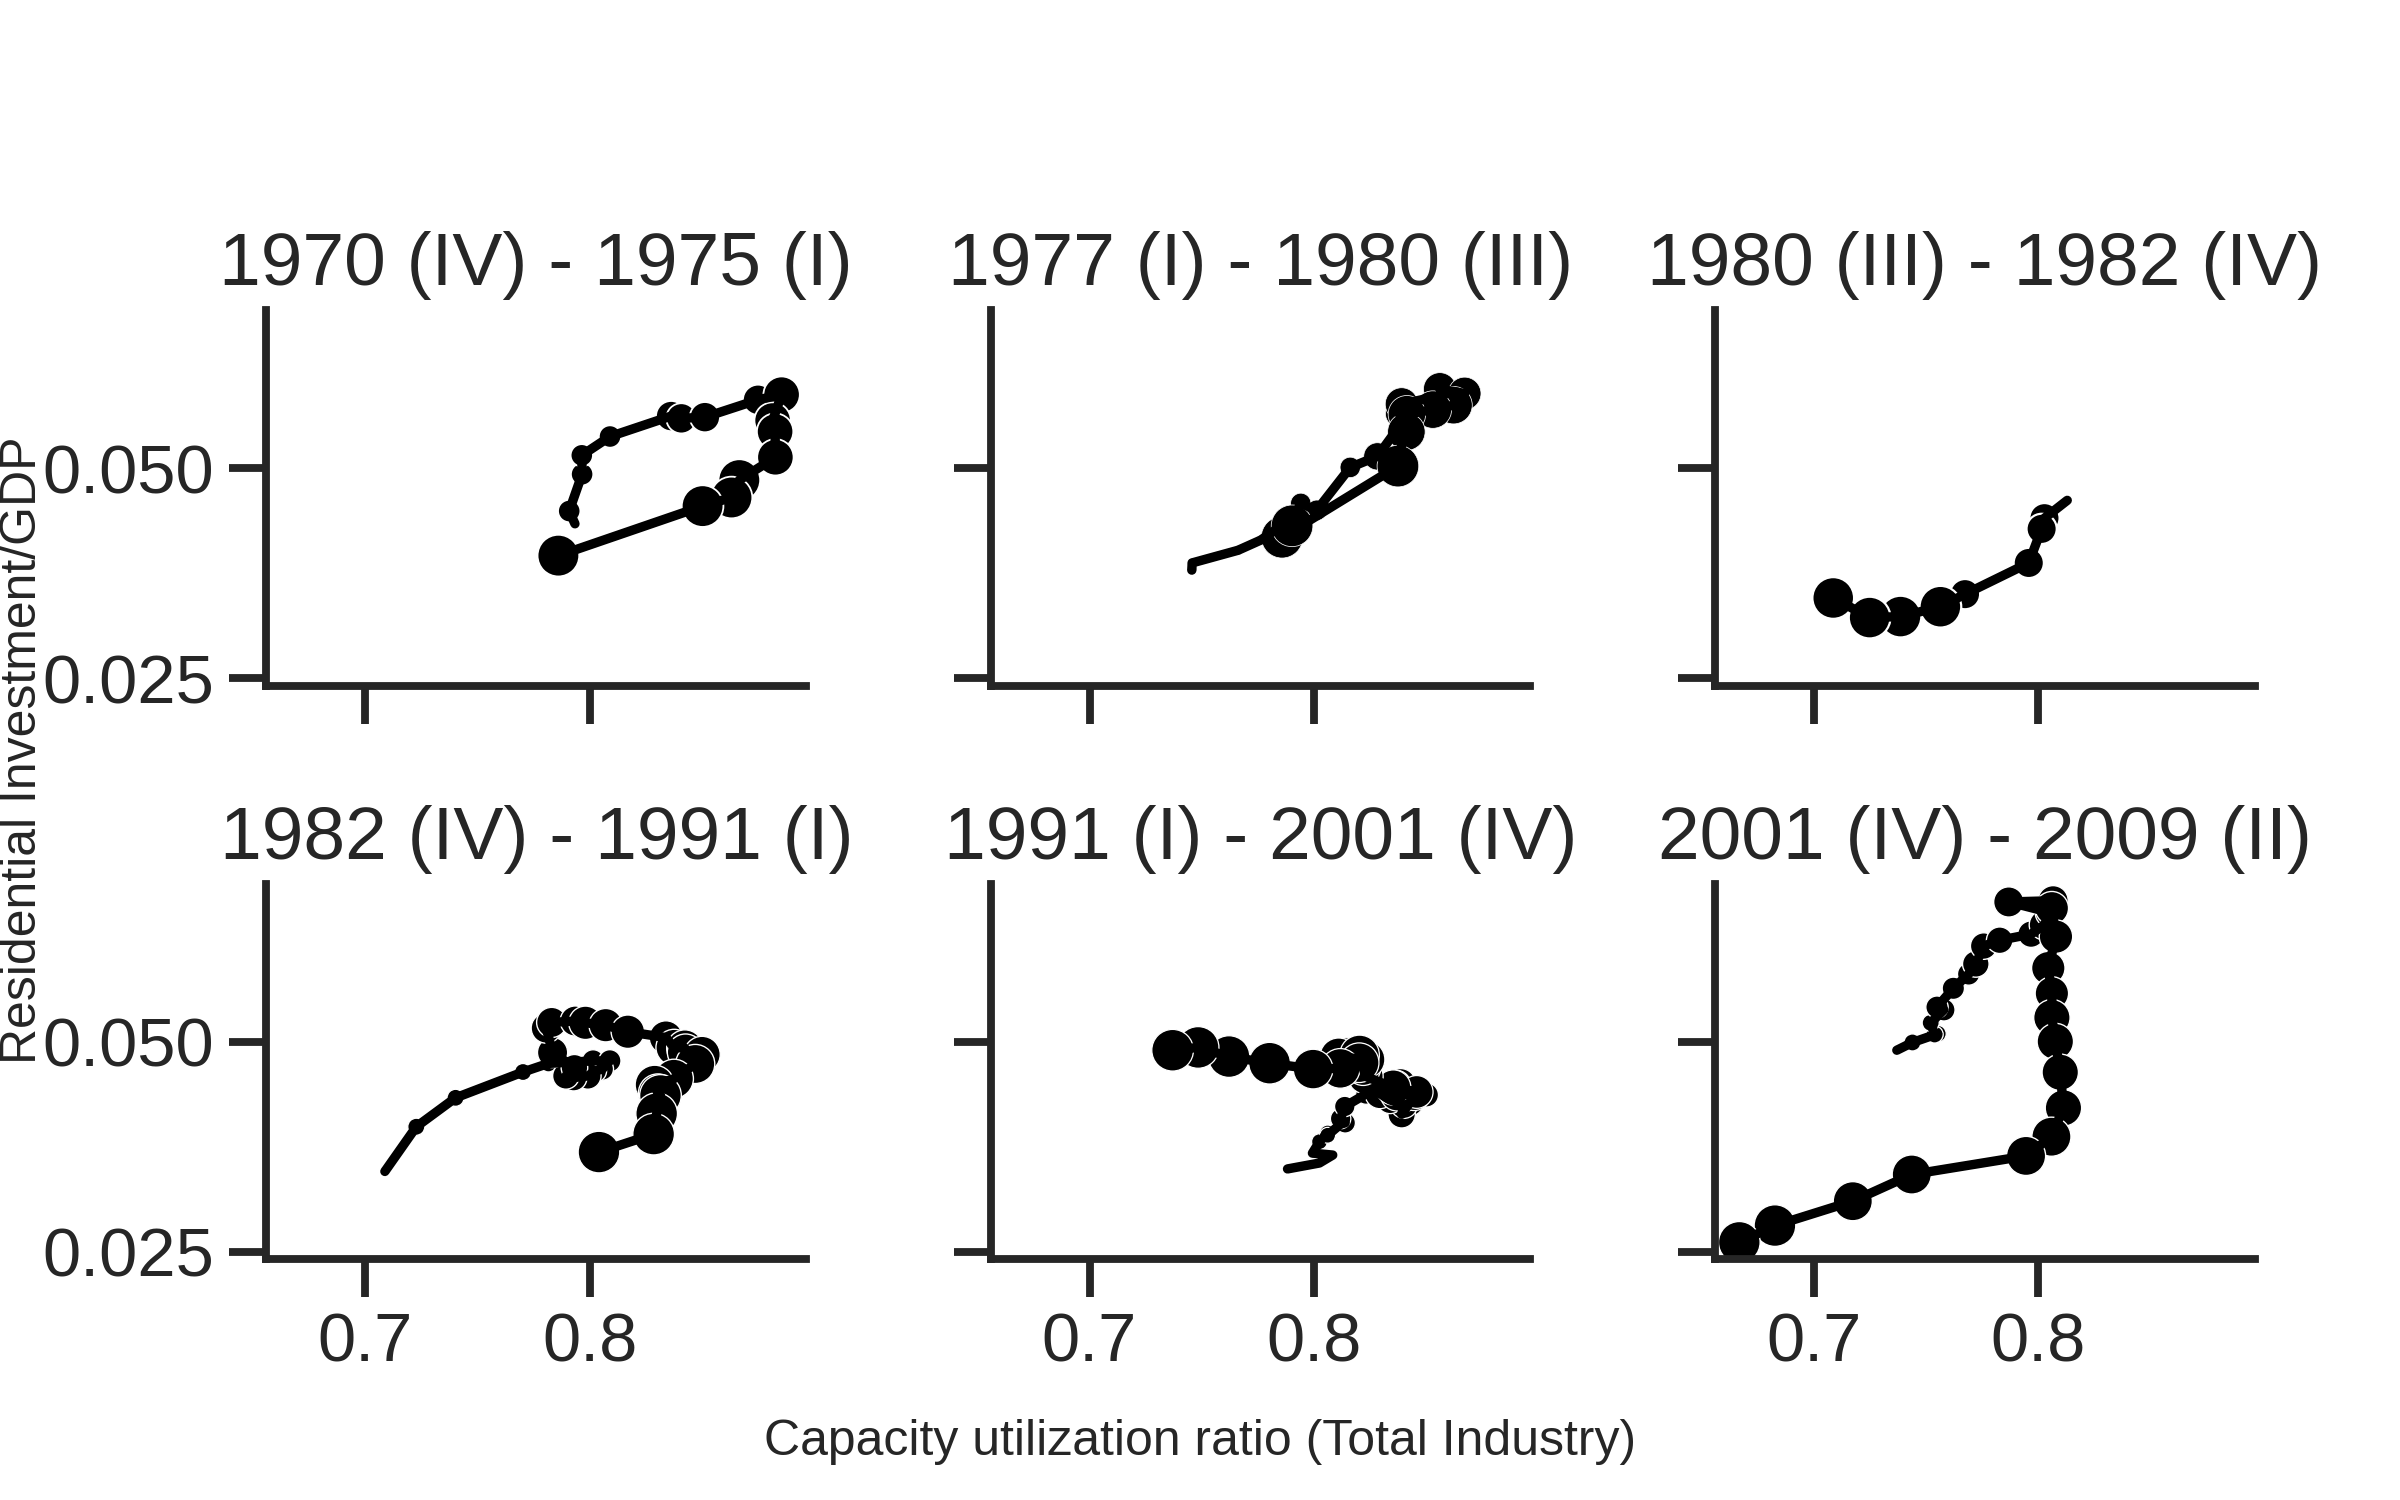
\includegraphics[width = 0.9\textwidth]{./figs/cycles.png}
    \label{fig:cycles}
    \caption*{\textbf{Source:} Federal Reserve Bank of St. Louis, authors’ elaboration.}
\end{figure}
Another key aspect of recent housing development is the  popularization of primary houses and concentration of secondary ones\footnote{According to \textcite{us_census_bureau_characteristics_2017}, a primary property is one that the owner has regular access to and, in the case of having more than one (secondary) property, it is the one that enjoys most of the time throughout the year. Secondary properties are those where:
(i) the owners reside part of the year only; (ii) it is at least 50 miles from the primary property and; (iii) cannot be subject to a rental agreement.}. The expansion of primary houses can be seen in Figure \ref{fig:concentration}, which shows the concentration curve from 1989 to 2010 by different types of properties (primary and secondary)\footnote{Concentration curves are drawn from the cumulative ordering of two distinct variables. The horizontal axis of Figure \ref{fig:concentration} contains the cumulative proportion of wealthy households while the vertical axis shows the accumulated proportion of a portion of this wealth (in this case, primary and secondary houses). Finally, to build the concentration curves, both axes are ordered by total wealth. Thus, unlikely the Lorenz curve, concentration curves are non-decreasing. As a consequence, it can cross the perfect equality line. For more details, see \textcite{Jann_Concentration_2016}.}. Based on these curves, it is possible to assess how concentrated a certain asset is by comparing it with perfect equality line\footnote{In 2010, for example,  up to 25\% of wealthy households owned 21.80\% of all primary houses. Moving on, households up to 50\%, 75\% and 90\% owned 61.30\%, 90.10\% and  95.30\% respectively while 2.9\% was not in the possession of any households.}\textsuperscript{,}\,\footnote{The higher and to the left a concentration curve is compared to the Lorenz curve, the less concentrated the asset is. In this case, the asset  is distributed in favor of the poorest strata of wealth. A concentration curve more to the right and below compared to the Lorenz curve indicates the opposite.}.

\begin{figure}[htb]
    \centering
        \caption{Concentration curves for primary and secoundary houses} 
    \includegraphics[width = 0.95\textwidth]{./figs/Concentration_Curve.png}
    \label{fig:concentration}
    \caption*{\textbf{Source:} Survey of Consumer Finance, authors’ elaboration.}
\end{figure}


A brief inspection of Figure \ref{fig:concentration} reveals that the years leading up to the Great Recession were characterized by the deconcentration of primary houses. In other words, poorer strata of the population now have a larger accumulated share of this type of asset. 
Since primary houses concern those that are used for purposes that are not necessarily speculative, there is a general increase in the demand for properties as final good. The same cannot be said about secondary houses whose concentration/distribution movement is not as marked as in the previous case. Since this type of property is not intended for regular use by its owner, a greater distribution of this asset suggests an increase in the demand for properties in the expectation of capital gains\footnote{This increase in demand for secondary houses may indicate --- but is not limited to --- an increase for speculative reasons. A vacation or rental home, for example, are non-speculative uses of a secondary house. Nevertheless, it is argued that there is a connection between secondary houses and speculation with real estate. It worth noting that the wealthiest households are not the main holders of this secoundary houses. According to Figure \ref{fig:concentration}, they accumulate less than 50\% of these properties over the analyzed period (see vertical axis).}.

\subsubsection{Conexão com a subseção seguinte}
\label{sec:orgc8af542}


\subsection{Housing bubble and residential investment}
\label{sec:org915a456}


After the Great Recession, the literature have analyzed the macroeconomic relevance of residential investment \cites{leamer_housing_2015}{fiebiger_semi-autonomous_2018}.
However, little progress has been made in understanding its theoretical determinants.
\textcite{teixeira_crescimento_2015} proposes the so-called houses own interest rate (\(own\)) in order to analyze the relation between residential investment, real estate inflation and interest rates during the U.S. housing bubble episode.
Estimated by deflating mortgages interest rate real estate inflation, this particular real interest rate is the most relevant for households since it is the real cost in real estate from buying real estate  \cite[p.~53]{teixeira_crescimento_2015}.
In short, this is the real interest rate that is relevant for house investors.
Figure \ref{propria_investo} shows how this  procedure is more adequate than a general price index deflation --- as \textcite[p.~143--6]{fair_macroeconometric_2013} does --- to describe residential investment growth rate\footnote{It is worth noting that during a housing bubble period, it is real estate inflation that governs own's interest rate dynamics. Therefore, the lower this rate is, the greater the capital gains (in real estate) for speculating with real estate will be. This negative relation between houses own interest rate and residential investment is shown in Figure \ref{propria_investo} in which this particular real interest rate has been gradually decreased over the real estate boom (2002-5).}.
Based on this concept, \textcite{petrini_demanda_2019} estimated an econometric model for the U.S. (1992 to 2019) and presents empirical evidence that the residential investment growth rate and houses own interest rate share a common negative long-run trend.
Furthermore, \textcite{petrini_demanda_2019} also reports a unidirectional long-run causality from houses own interest rate to residential investment growth rate.

EXPLICAR TAXA PRÓPRIA


\begin{figure}[htb]
	\centering
	\caption{Residential investment growth rate vs. Houses Own interest rate}
	\label{propria_investo}
	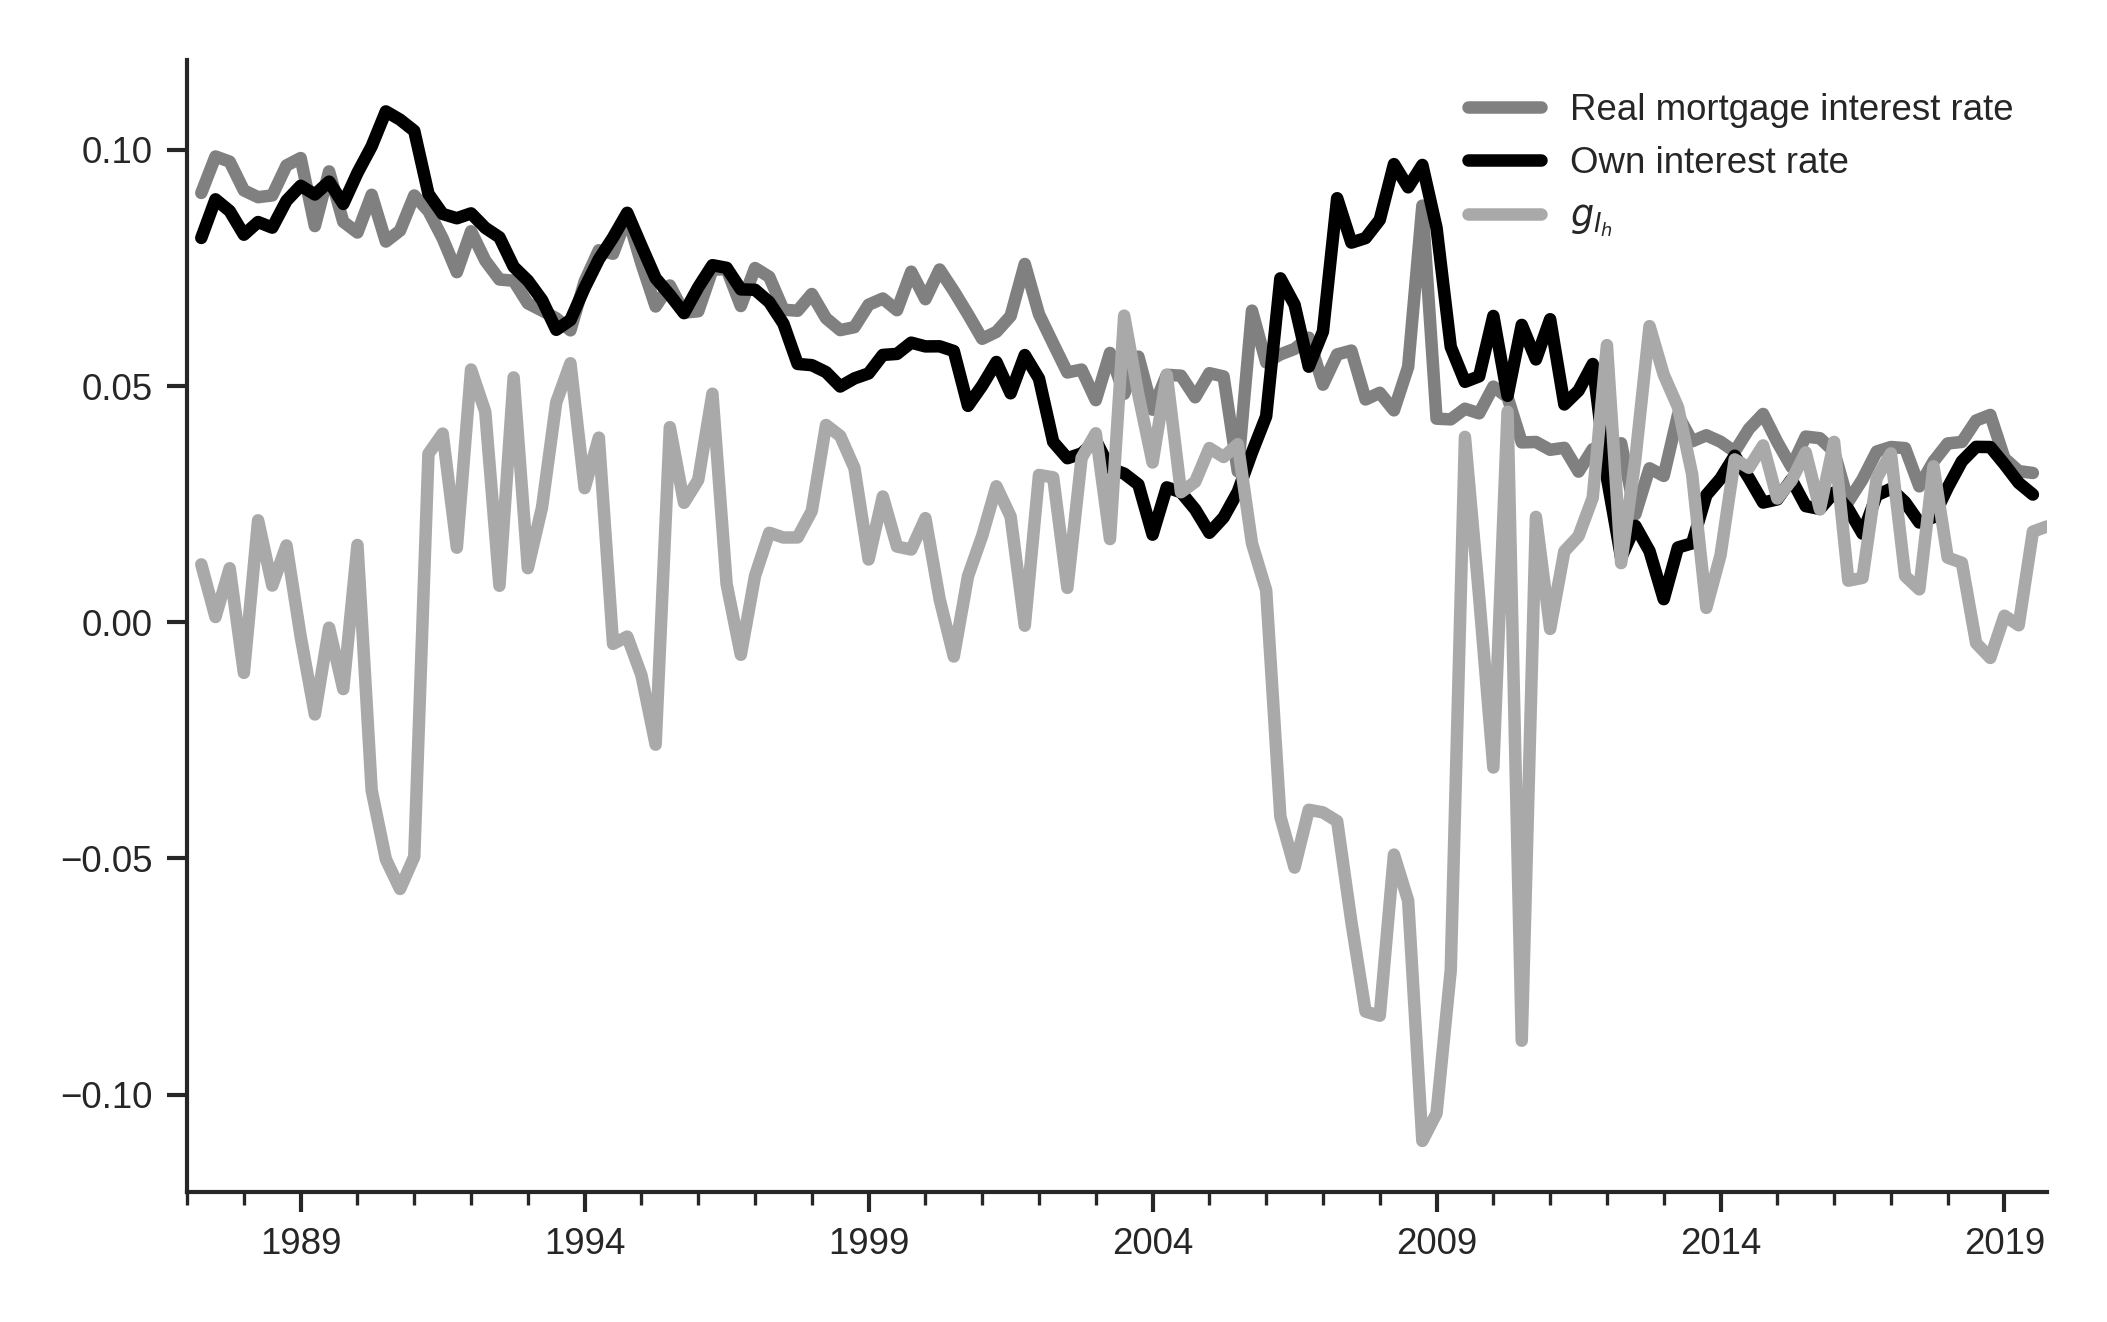
\includegraphics[width=.8\textwidth]{./figs/Own_gI}
	\caption*{\textbf{Source:} U.S. Bureau of Economic Analysis, Authors' elaboration}
\end{figure}





In summary, what we intended to show is that one cannot analyze the U.S. business cycle properly without considering residential investment and asset bubbles together.


\section{A Sraffian supermultiplier SFC model with residential investment}
\label{sec:orgdb0d305}
\label{sec:Model}
\subsection{General equations}
\label{sec:org974e94e}

Our model is the most parsimonious as possible: a closed capitalist economy without government sector. Output (\(Y\)) is determined by  a fixed combination of a homogeneous labor (\(L\)) input with homogeneous fixed business capital (\(K_f\)). 
For simplicity, we put technological progress, depreciation and goods inflation aside so investment is presented in net terms and all variables --- except for houses --- are measured in real terms.
Assuming a Leontief production function and that growth is not constrained by labor scarcity, full capacity output (\(Y_{FC}\)) is
determined by firms' capital stock:
\begin{equation}
\label{_Leontieff}
    Y_{FC} = \min (Y_L, Y_K)
\end{equation}
\begin{equation}
\label{_YFC}
    Y_{FC} = \frac{K_{f_{-1}}}{v}
\end{equation}
\begin{equation}
\label{_u}
    u = \frac{Y}{Y_{FC}}
\end{equation}
where \(Y_L\) and \(Y_K\) stands for full employment and full capacity output respectively, \(v\) is exogenous capital-output ratio and \(u\) is utilization rate.

We further assume an economic structure composed by both workers (denoted by \(w\)) and capitalists (denoted by \(k\)) households\footnote{In accordance with \textcite{albanesi_credit_2017}, we consider that only the latter invest in real estate and are not credit constrained.}.
Thus, demand-determined output level (\(Y\))  is the sum of workers and capitalists consumption (\(C_w\) and \(C_k\) respectively) and both households and firms investment (\(I_h\) and \(I_f\) respectively) and only the latter creates capacity to the business sector of the economy:
\begin{equation}
\label{_Ct}
    C = C_w + C_k
\end{equation}
\begin{equation}
\label{_It}
    I_t = I_f + I_h
\end{equation}
\begin{equation}
\label{_Y}
    Y = \overbrace{[C_w + \underbrace{C_k + I_h}_{\text{Capitalists}}]}^{\text{Households}} + \overbrace{[I_f]}^{\text{Firms}}
\end{equation}

In other words, from institutional sectors perspective, household expenditures have two components (consumption and residential investment) and firms just one (non-residential investment). 
Only non-residential investment creates productive capacity. 
So, the novelty of this model is the inclusion of a second investment component all made by household sector and held by capitalists households for simplicity. 
Therefore, this economy produces two types of real assets: firms productive capital (\(K_f\)) and households housing (\(K_h\)):
\begin{equation}
    \label{_K}
    K = K_f + K_h
\end{equation}

Denoting the houses share in total real assets as \(k\), we can rewrite equation \ref{_K} as:
\begin{equation}
\label{_k}
    k = \frac{K_h}{K}
\end{equation}
$$
K = (1-k)\cdot K + k\cdot K
$$

We further assume an exogenous functional income distribution. 
Following Sraffian strands, profit-share is determined both by historical-institutional factors and class struggle.
As a consequence, we define total wages (\(W\), Eq. \ref{_W}) as a function of wage-share (\(\omega\)):

\begin{equation}
\label{_W}
    W = \omega\cdot Y
\end{equation}

Table \ref{Matriz_Estoques} presents the balance sheet matrix for all institutional sectors. 
Capitalists households hold financial wealth as bank deposits (\(M\)) and residential investment is financed by mortgages (\(MO\)).
Capitalists' total net wealth (\(NW_{k}\)) is the sum of their net financial wealth (\(V_{k}\)) and real assets (\textit{i.e.} housing, \(K_h\)). 
Table  \ref{Matriz_Fluxos} presents both transactions flows and the flow of funds matrix. 
This table shows all economic relations between institutional sectors ensuring that there is no  ``black holes''
so all financial and real transaction are explicitly defined \cite{macedo_e_silva_peering_2011}.

In this model, capitalist consumption (\(C_k\)) is fully autonomous and financed by loans (\(L_{k}\)) while workers consumption (\(C_w\)) is fully induced by their wages.
We assume that workers expend what they earn while capitalists earn what they expend, so workers financial and real wealth are both null.
Firms finance their investment primarily by undistributed profits (\(FU\)) and the residual by bank loans (\(L_f\)) --- thus they do not hold deposits. 
Banks create credit \textit{ex nihilo} and then collect the deposits, paying the same interest rate that they charge.
On the following subsections, we will present the equations of each of these institutional sectors.



\begin{table}[H]
\centering
\caption{Balance Sheet matrix}
\label{Matriz_Estoques}
\begin{tabular}{lccccc}
\hline
\hline
                          & Workers & Capitalists      & Firms        & Banks  &    $\sum$ \\ \hline

Deposits & & $+M$ & & $-M$ & 0\\
Loans& &$-L_{k}$ &$-L_f$& $+L$ & 0\\
Mortages & &$-MO$&  & $+MO$ & 0\\\hline
$\sum$ Net Financial Wealth &--- &$V_{k}$&$V_f$&$V_b$& $0$\\\hline
Capital & & &$+K_f$&  & $+K_f$\\
Houses & &$+K_{hd}$& &   & $+K_h$\\\hline
$\sum$ Net Wealth &---&$NW_{k}$&$NW_f$&$NW_b$& $+K$\\
\hline
\hline
\end{tabular}%
\caption*{\textbf{Source:} Authors' Elaboration}
\end{table}


\begin{table}[H]
\centering
\caption{Transactions flow matrix and flow of funds
}
\label{Matriz_Fluxos}
\resizebox{\textwidth}{!}{%
\begin{tabular}{lccccccc}
\hline
\hline
& Workers
& \multicolumn{2}{c}{Capitalists}
& \multicolumn{2}{c}{Firms}                        
& Banks       & Total    \\ \cline{3-4}\cline{5-6}
& &
Current & Capital & 
Current & Capital     & 
&       $\sum$ \\ 
Consumption                       &$-Cw$&$-C_k$& & $+C$& & & 0\\
Non-residential Investment                   & & & &$+I_f$&$-I_f$ & & 0\\
Residential Investment       &  & &$-I_h$&$+I_h$& & & 0\\
\textbf{{[}Output{]}}   & & & &{[}$Y${]}& & & {[}$Y${]}\\
Wages                        &$+W$&& &$-W$& & & 0\\
Profits                      & &$+FD$& &$-FT$&$+FU$& & 0\\
Deposits interest rate         & &$+r_m\cdot M_{-1}$& && &$-r_m\cdot M_{-1}$& 0\\
Loans interest rate         & &$-r_l\cdot L_{k_{-1}}$& &$-r_l\cdot L_{f_{-1}}$& &$+r_l\cdot L_{-1}$& 0\\

Mortages interest rates         & &$-r_{mo}\cdot MO_{-1}$& && &$+r_{mo}\cdot MO_{-1}$& 0\\\hline
\textbf{Subtotal}           &---&$+S_h$&$-I_h$& &$+NFW_f$&$+NFW_b$& 0\\\hline
Change in deposits     & &$-\Delta M$& & & &$+\Delta M$& 0\\
Change in mortgages     & & &$+ \Delta MO$& & &$-\Delta MO$& 0\\
Change in loans     & &$+\Delta L_{k}$&&$+\Delta L_f$& &$-\Delta L$& 0\\
\textbf{Total} & & 0 & 0 & 0  & 0  & 0  & 0\\
\hline
\hline
\end{tabular}%
}
\caption*{\textbf{Source:} Authors' Elaboration}
\end{table}


\subsection{Firms}
\label{sec:org75823ba}

In order to produce, firms purchase capital goods (\(-I_f\) in capital account) and hire workers, whom total remuneration is the economy wage bill. 
Their total profits (\(FT\)) are a residual between sales (\(Y\)) and total wages (\(W\)). 
Firms retain part (\(\gamma_F\)) of profits net of interest payments (\(FU\)) --- to reinvest --- and distribute the rest to capitalists (\(FD\)):

\begin{equation}
\label{_FT}
    FT = Y - W = FD + FU
\end{equation}
\begin{equation}
    FU = \gamma_F\cdot (FT - r_l\cdot L_{f_{-1}})
\end{equation}
\begin{equation}
    FD = (1-\gamma_F)\cdot (FT - r_l\cdot L_{f_{-1}})
\end{equation}

Firms (non-residential) investment is fully induced by the level of effective demand (Eq. \ref{_If}), and its growth rate changes accordingly to the capital stock adjustment principle \cite{freitas_growth_2015}.
Equation \ref{_h} in one simple way to describe this mechanism.
According to it, the marginal propensity to invest (\(h\)) endogenously adjust the discrepancies between actual and normal utilization rates (\(u\) and \(u_N\), respectively). To do so, the adjustment parameter (\$\(\gamma\)\_u) must sufficiently small and non-negative\footnote{The size of this parameter guards a fundamental relation to the stability of the model, as shown by \textcite{freitas_growth_2015}.}. 
As a consequence, productive capacity gradually reacts to effective demand movements.

\begin{equation}
\label{_If}
    I_f = h_{t-1}\cdot Y
\end{equation}
\begin{equation}
\label{_h}
    \Delta h = h_{t-1}\cdot \gamma_u\cdot (u - u_N)
\end{equation}
\begin{equation}
    \Delta K_f = I_f
\end{equation}


Firms finance part of investment that exceeds undistributed profits by bank loans, paying an interest rate on it (\(r_l\)) charged by the banks. 
We assume an elastic supply of credit for investment. 
Moreover, tables \ref{Matriz_Estoques} and \ref{Matriz_Fluxos} show firms net wealth (\(NW_f\)) and net financial balance (\(NFW_f\)) explicitly:

\begin{equation}
\label{_Lf}
    \Delta L_f = I_f - FU
\end{equation}
$$
r_g = \frac{1-\omega\cdot u}{v}
$$
$$
r_n = r_g - r_l\cdot\frac{L_{f_{-1}}}{K_f}
$$
\begin{equation}
    NFW_f = FU - I_f
\end{equation}
\begin{equation}
    NW_f = K_f - L_f
\end{equation}
where \(r_g\) and \(r_n\) denotes gross and net profit rate respectively.


\textbf{TODO:} Substituir letra da taxa de lucro por outra.

\subsection{Banks}
\label{sec:org9539a2d}

As in most part of SFC literature, banks do not have an active role in this model.
They create money as credit is demanded and just after they collect deposits \cite{le_bourva_money_1992}. 
Firms finance part of their investment with credit (\(L_f\)) and capitalists households finance all their residential investment by mortgages (\(MO\)) and consumption by loans (\(L_{k}\)), as already mentioned. 
Each operation has its own interest rate defined by a spread (\(\sigma_l\) and \(\sigma_{mo}\)) over deposits interest rate (\(r_m\)) exogenously determined by banks.
For simplicity, we assume null bank spreads so interest rate on mortgages and on loans
are the same as on deposits.
Banks net balances (\(NFW_b\)) are defined by interests received net of interests payments. 
As those interests are the same, banks net wealth is necessarily zero (see table \ref{Matriz_Estoques}) and deposits are residuum:

\begin{equation}
L = L_f + L_{k}
\end{equation}
\begin{equation}
    r_l = (1+\sigma_l)\cdot r_m
\end{equation}
\begin{equation}
    r_{mo} = (1+\sigma_{mo})\cdot r_m
\end{equation}
\begin{equation}
    r_m = \overline r_m
\end{equation}
\begin{equation}
    NFW_b = r_{mo}\cdot MO_{-1} + r_l\cdot L_{-1} - r_m\cdot M_{-1}
\end{equation}
$$
NFW_b = \Delta MO + \Delta L - \Delta M
$$
\begin{equation}
    NW_b = V_b \equiv 0
\end{equation}
\begin{equation}
\label{_M}
    \Delta M = \Delta L + \Delta MO
\end{equation}

\subsection{Households}
\label{sec:orgb5a441f}

\subsubsection*{Workers}
\label{sec:orgd3e86ef}
As mentioned before, we assume that workers expend (\(C_w\)) what they earn (\(W\)). 
For simplicity, we consider that wages are the only source of income workers' disposable income (\(YD_{w}\)) and do not have access to consumption loans, so worker' saving (\(S_{hw}\)) are null.
Therefore, accordingly to our hypothesis, workers' do not hold both net financial and total wealth.

\begin{equation}
C_w = W
\end{equation}
\begin{equation}
YD_w = W
\end{equation}
\begin{equation}
S_{w} = YD_w - C_w
\end{equation}
$$
S_{w} = 0
$$
\begin{equation}
NFW_{w} = S_{w} = 0
\end{equation}
\begin{equation}
V_{w} = 0
\end{equation}

\subsubsection*{Capitalists}
\label{sec:org71c7f46}
This is the most complex institutional sector of our model. 
We assume consumption (\(C_k\)) is fully-autonomous and financed by loans (\(L_{k}\)). 
Disposable income (\(YD_k\)) is the sum of distributed profits and received interests on deposits, net of interests payments
on both mortgages and loans.
Capitalists savings (\(S_{k}\)) are disposable income net of consumption.
At odds with SFC literature, savings are not equal to net balance (\(NFW_{k}\)) since we have included residential investment as in Equation \ref{NFWh}.

\begin{equation}
\Delta L_{k} = C_k
\end{equation}
\begin{equation}
    \label{EqYD}
    YD_k = FD + \overline r_m\cdot M_{-1} - r_{mo}\cdot MO_{-1} - r_{l}\cdot L_{k_{-1}}
\end{equation}
\begin{equation}
    \label{EqSh}
    S_{k} = YD_k - C_k
\end{equation}
\begin{equation}
\label{NFWh}
    NFW_{k} = S_{k} - I_h
\end{equation}


As mentioned before, capitalist households are the only institutional section investing in real estate which is financed by mortgages as in equation (\ref{EqMO}). Next, we present residential investment growth rate (\(g_{I_h}\)) as determined by houses own interest rate (\(own\), equation \ref{_own}) as introduced by \textcite{teixeira_crescimento_2015} and discussed in section \ref{sec:empirical}.


\begin{equation}
    \label{EqMO}
    \Delta MO = I_h
\end{equation}





\begin{equation}
    I_h = (1 + g_{I_h})\cdot Ih_{-1}
\end{equation}
\begin{equation}
\label{g_Z_own}
g_{I_h} = \phi_0 - \phi_1\cdot own
\end{equation}

\begin{equation}
\label{_own}
own = \left(\frac{1+r_{mo}}{1+\pi}\right) -1
\end{equation}
$$
\pi = \frac{\Delta p_h}{p_{h_{t-1}}}
$$
where \(\pi\) stands for real estate inflation, \(\phi_0\) represents long-term determinants (\emph{e.g.} demographic factors, housing and credit policies, etc.) while \(\phi_1\) captures the demand for real estate arising from expectations of capital gains resulting from speculation with the existing dwellings stock. 

Accordingly to our hypothesis, nominal (\(V_{nk}\)) and real net wealth (\(V_{k}\)) are distinguished only by the inclusion of real estate price (\(p_h\)) and are defined as follows:
\begin{equation}
V_{k} = K_{hd} + M - L_{k} - MO
\end{equation}
\begin{equation}
V_{nk} = K_{hd}\cdot p_h + M - L_{k} - MO
\end{equation}


In order to fulfill our goals, we employ \citeauthor*{freitas_baseline_2020}'s \citeyear{freitas_baseline_2020} procedure in which NCC autonomous expenditure (\(Z\)) composition (\(R\)) remains unchanged. Thus, we can express capitalists total consumption as follows:

\begin{equation}
\label{_Z}
Z = C_k + I_h
\end{equation}
$$
\frac{C_k}{Z} + \frac{I_h}{Z} = R + (1-R)
$$
which allows us to rewrite both NCC and autonomous consumption in terms of residential investment (Eq. \ref{Z_Ih}):
\begin{equation}
\label{_Ck}
    C_k = R\cdot Z
\end{equation}
\begin{equation}
\label{Z_Ih}
Z = \frac{I_h}{(1-R)}
\end{equation}

\begin{equation}
\label{C_kZ}
C_{k} = I_h\cdot \frac{R}{(1-R)}
\end{equation}

Finally,  we can describe NCC autonomous expenditure growth rate as follows:
\begin{equation}
\label{g_Z}
g\textsubscript{C\textsubscript{k}} = g\textsubscript{Z} = g\textsubscript{I\textsubscript{h}} = \(\phi\)\textsubscript{0} - \(\phi\)\textsubscript{1}\(\cdot\) own
\end{equation}

In this section, we presented a fully-specified parsimonious model to connect asset bubbles with aggregate demand. It worth mentioning that, although simplified, our hypotheses are supported data as discussed in Section. 
%Following textcites:teixeira_crescimento_2015,petrini_demanda_2019, we specify a econometrically significant residential investment growth rate function which allows us to include housing bubbles in the SMM model.
On the next Section, we present the short-run and fully-adjusted position dynamics in order to show the particularities of a model with two types of capital stock in the presence of asset bubble.



\section{Short and long-run equilibria}
\label{sec:org1c07671}
\label{sec:runs}
In this Section, we show the implications residential investment inclusion into a SSM-SFC model. First, we present the short-run dynamics and then move to the fully-adjusted position (denoted by \(\star\)).
\subsection{Short-run good market equilibrium}
\label{sec:org927ea54}
\label{short}

In this model, real output (equation \ref{_Y}) is the sum of household consumption (equation \ref{ConsumoTotal}) and both types of investment (equation \ref{_It}). 
If we replace equations \ref{_W} and  \ref{_If} into \ref{_Y} and considering equation \ref{_Z} we get the short-run GDP level:

\begin{equation}
\label{Y_nivel}
Y_t = \frac{Z_t}{1 - h_t - \omega}
\end{equation}
and replacing Equation \ref{Z_Ih} in the previous one
\begin{equation}
\label{Y_Ih}
Y_t = \frac{I_h}{(1-R)(1 - h_t - \omega)}
\end{equation}
Next, dividing equation \ref{Y_Ih} by \ref{_YFC} and rearranging, we get the short-run equilibrium utilization rate (Eq \ref{short_u})


\begin{equation}
\label{u_to_k}
u_t = \frac{I_h}{(1-R)(1-h_t - \omega)}\frac{v}{K_{f_{t-1}}}
\end{equation}
$$
u_t = \frac{I_{h_{t-1}}\cdot (1 + g_{I_h})}{(1-R)(1-h_t - \omega)}\frac{v}{K_{f_{t-2}}\cdot (1+g_{K_{t-1}})}
$$

\begin{equation}
\label{short_u}
u_t = \frac{v}{(1-R)(1-h_t - \omega)}\frac{I_{h_{t-1}}}{K_{f_{t-2}}}\frac{(1 + g_{I_h})}{(1+g_{K_{t-1}})}
\end{equation}


Finally, replacing residential investment growth rate by Equation \ref{g_Z_own}


\begin{equation}
\label{short_u}
u_t = \frac{v}{(1-R)(1-h_t - \omega)}\frac{I_{h_{t-1}}}{K_{f_{t-2}}}\frac{(1 + \phi_0 - \phi_1\cdot own_t)}{(1+g_{K_{t-1}})}
\end{equation}

Before moving towards the traverse, we revisit Equation \ref{u_to_k} in order to present houses share on total capital stock (\(k\))\footnote{As we will see on section \ref{long}, this ratio guards a special relation with marginal propensity to invest in the fully-adjusted position.}.  To do so, we express firms' capital in terms of houses. 
$$
u_t = \frac{I_h}{(1-R)(1-h_t - \omega)}\frac{v}{(1-k)\cdot K_{t-1}}
$$
Finally, dividing both sides of equation \ref{u_to_k} by houses and after some algebraic manipulations, we get firms' capital-to-houses ratio (Equation \ref{k_short})\footnote{The intermediate steps to obtain Equation \ref{k_short} are
$$
u_t = \frac{v}{(1-R)(1-h_t - \omega)}\frac{I_h}{K_{HD_{t-1}}}\frac{1}{(1-k)}\frac{K_{HD_{t-1}}}{K_{t-1}}
$$
$$
u_t = \frac{v\cdot g_{I_h}}{(1-R)(1-h_t - \omega)}\frac{k}{(1-k)}
$$
$$
1-k = \frac{v\cdot g_{I_h}}{(1-R)(1-h_t - \omega)}\frac{k}{u}
$$
then
$$
\frac{1-k}{k} = \frac{v\cdot g_{I_h}}{(1 - h_t - \omega)\cdot u_{t}}
$$}

$$
u_t = \frac{I_h}{(1-R)(1-h_t - \omega)}\frac{v}{(1-k)\cdot K_{t-1}}\frac{K_{HD_{t-1}}}{K_{HD_{t-1}}}
$$

$$
k = \frac{u_t\cdot (1-R)\cdot (1-h_t - \omega)}{g\cdot v + u_t\cdot  (1-R)\cdot (1-h_t - \omega)}
$$

\begin{equation}
\label{k_short}
k = \frac{(1-R)\cdot (1-h_t - \omega)}{\frac{g\cdot v}{u_t} + (1-R)\cdot (1-h_t - \omega)}
\end{equation}


\subsection{Analytical Traverse}
\label{sec:orgbb3e8dd}

\textbf{Nota:} Optei por chamar de ``Analytical Traverse'' (não sei se faz sentido/existe) porque ainda vamos simular e estas relações não estão exatamente expressas ali.

\textbf{Nota:} Começar descrevendo a partir da diferença entre \(g\) e \(g_K\) e subsequente processo de reajustamento

In this subsection, we present traverse following \textcite{freitas_growth_2015}\footnote{It worth mentioning that we addopt a slightly different concept of medium-run from \textcite{freitas_growth_2015}. That is why we chose to refer to is as traverse as usual in SFC literature. \textcite{freitas_growth_2015} describes medium-run as the theoretical moment when expenditures growth rates converges to the NCC growth rate (\(g_{I_h}\) in our case). However, as we employ numerical simulations, that equality could not occur during the traverse. That been said, the medium-run is defined as the moment in which the capacity ratio is not equal to the normal one while the firms' investment is still adjusting according to changes in marginal propensity to invest (\(h\neqh^\star\)).}.
According to equation \ref{short_u}, when aggregate demand and capacity output growth at different rates, capacity utilization will change. 
This discrepancy triggers marginal propensity to invest adjustment mechanism (see Equation \ref{_h}). 
During the adjustment process, both supermultiplier and NCC autonomous expenditure share on GDP changes.
Equation \ref{g_medium} presents aggregate demand during the traverse:

\begin{equation}
\label{g_medium}
g_t = g_{Z} + \frac{\Delta h}{1 - \omega - h_{t}}
\end{equation}
This process continues as long as GDP growth rate moves towards NCC autonomous expenditure growth rate (in this case, residential investment and capitalist consumption). On the following subsection, we analyze the fully-adjusted positions values and steady state stock/flow ratios.


\subsection{Fully-adjusted position}
\label{sec:org1b0ccc1}
\label{long}

As mentioned before, endogenous firms’ marginal propensity to invest reacts to discrepancies between the utilization rate and the normal one.  This adjustment process continues until actual a normal capacity utilization rate are equal:

$$
u \to u^{\star}  = u_N \Leftrightarrow g \to g^{\star} = g_Z
$$
and (endogenous) fully-adjusted position marginal propensity to invest will be:


\begin{equation}
\label{h_long}
h^{\star} = g^{\star}\cdot \frac{v}{u^{\star}}
\end{equation}

Next, we move towards the analysis of the particularities of our model:  one of the NCC autonomous expenditures also contributes to total capital stock.  
Replacing Equation \ref{h_long} in \ref{k_short}, we obtain fully-adjusted position of the ratio between houses and total capital stock (denoted by \(k^\star\)):

$$
k^{\star} = \frac{(1-R)(1-h^\star - \omega)}{h^\star + (1-R)(1-h^\star - \omega)}
$$
\begin{equation}
\label{k_long}
k^{\star} = 1 - \frac{h^{\star}}{h^\star + (1-R)(1-h^\star - \omega)}
\end{equation}



Before moving on to the numerical simulations, we present some steady state stock/flow ratios in order to shed some light in the dynamic process of the model. Dividing Equation \ref{_Lf} by firms' lagged capital stock and making some algebraic manipulation, we obtain steady state loans' ratio to capital stock (\(\ell^{\star}\), Equation \ref{firm_ratio}):

$$
\Delta \left(\frac{L_{f}}{K_{f}}\right) = \frac{I_{f} - FU}{K_{f}} - \ell^{\star}_{f}\cdot g^{\star}  = 0
$$


\begin{equation}
\label{firm_ratio}
l^\star_f = \frac{g^\star\cdot v - \gamma_F\cdot u^\star \cdot (1-\omega)}{v\cdot (g^\star - \gamma_F\cdot r_m)}
\end{equation}

Next, we rewrite capitalists autonomous expenditure in terms of residential investment (see Equation \ref{C_kZ}). 
Then, we  present capitalists' loans to houses stock ratio (Equation \ref{capitalist_ratio}):

$$
\Delta \left(\frac{L_k}{K_{HD}}\right) = \frac{C_k}{K_{HD}} - \ell^{\star}_{k}\cdot g^{\star} = 0
$$

\begin{equation}
\label{capitalist_ratio}
l^\star = \frac{R}{1-R}
\end{equation}

The same procedure can be applied to find mortgage to house stock ratio (\(mo^{\star}\), Equation \ref{mortgage_ratio}):
$$
\Delta \left(\frac{MO}{K_{HD}}\right) = \frac{\Delta MO}{K_{HD}} - mo^{\star}\cdot g^{\star} = 0
$$

\begin{equation}
\label{mortgage_ratio}
mo^\star = 1
\end{equation}
Thus, adding Equations \ref{capitalist_ratio} and \ref{mortgage_ratio} and, we get capitalists' total debt in terms of houses (\(d^\star\) Equation \ref{debt_ratio})

$$
d^\star = 1 + \frac{R}{1-R}
$$

\begin{equation}
\label{debt_ratio}
d^\star = \frac{1}{1-R}
\end{equation}

Finaly, we can express deposits share on total capital stock (\(m^{\star}\)) in terms of previous stock/flow ratios:

$$
\frac{M}{K} = \frac{MO + L_k + L_f}{K}
$$
$$
\frac{M}{K} = \frac{MO}{K_{HD}}\cdot \frac{K_{HD}}{K} +  \frac{L_k}{K_{HD}}\cdot \frac{K_{HD}}{K} +  \frac{L_f}{K_{f}}\cdot \frac{K_{f}}{K}
$$

\begin{equation}
\label{M_long_intermediate}
m\textsuperscript{\(\star\)} = mo\textsuperscript{\(\star\)}\(\cdot\) k\textsuperscript{\(\star\)} + \(\ell\)\textsuperscript{\(\star\)}\textsubscript{k}\(\cdot\) k\textsuperscript{\(\star\)} + \(\ell\)\textsuperscript{\(\star\)}\textsubscript{f}\(\cdot\) (1-k\textsuperscript{\(\star\)})
\end{equation}

Before moving on to the numerical simulations, it worth noting that --- besides its counterintuitivity --- the decrease of \(k^{\star}\) as a result of the increase of residential investment growth rate (reported in equations \ref{partial_phi0} and \ref{partial_pi} in Appendix \ref{append:Solution}) is in line with the SSM.
Since firms' investment grows (temporally) at a higher pace than NCC autonomous expenditures, it has only a level effect on capital stock.
As usual, changes in income distribution affects GDP temporally.
However, it has permanent effects over capital stock composition as a result of this level effect reported before (equation \ref{partial_omega}).


\section{Numerical Simulations}
\label{sec:org01411db}
\label{sec:Experiments}
\label{sec:Experiments}


In this Section, we present the results of the following experiments: 
    (i) wage-share decrease;
    (ii) real estate inflation and;
    (iii) deposits interest rate increase.
In order to evaluate if our model is able to reproduce some stylized facts, we introduce U.S. houses own rate of interest observed data (from 1992 to 2019) into our numerical simulation.
Before we move foward, it worth mentioning that we use \citeauthor*{fazzari-2020-deman-led}'s  \citeyear{fazzari-2020-deman-led} parameter values callibrated for the U.S. economy for a similar time range (from 1980 to 2016).
Our first experiment assess if income distribution affects fully-adjusted position growth rates temporal --- as in \textcite{mandarino-2020-worker-debt} --- or persistently ---  as in \textcite{brochier_supermultiplier_2018}.
Real estate inflation increase experiment is motivated by recent US experience (from 1992 to 2019) as discussed in Section \ref{sec:empirical} while the last simulation aims to evaluate indebtedness stability.
Table \ref{tab:param} in Appendix \ref{append:Data} presents the parameters of simulation and Table \ref{ResumoChoques} compare each result to baseline.
\subsection{Wage-share decrease}
\label{sec:org67b6e7f}
\label{sec:Exp1}

A wage-share decrease has a temporary negative impact both in GDP level and capacity utilization rate due to changes on the supermultiplier (see Figure \ref{fig:results_1}).
So, aggregate demand growth level is temporarily lower than baseline as a result of the lower supermultiplier.
As a consequence of this negative level effect, both accumulation growth rate and marginal propensity to invest temporaly decline while NCC autonomous expenditures share on GDP increases.
Since NCC autonomous expenditure growth rate remains unchanged and its share on GDP increases, aggregate demand grows faster than accumulation rate.
As a result, capacity utilization is higher than the normal one.
During the traverse, marginal propensity to invest endogenously adjust to discrepancies between actual and normal utilization rates.
Consequently, non-residential investment growth rate increases faster than aggregate demand.
This endogenous adjustment process continues as long as actual capacity utilization rate is different from the normal one.
In summary, we report standards SSM model results:
    (i) marginal propensity to invest decrease is temporally and returns to baseline level;
    (ii) utilization rate moves towards normal one;
    (iii) supermultiplier decreases and autonomous expenditure share increases due to GDP decline and; 
    (iv) since autonomous expenditure growth rate does not change, distribution effects on growth rates are temporary. 


Despite temporary effects in growth rate, wage-share decrease has a permanent effect in house share on total capital stock (see Equation \ref{k_long} and Figure \ref{fig:results_2}).
As a consequence of the initially lower accumulation rate, total capital stock also grows at a temporarily lower rate.
However, since residencial investment growth rate remains unchanged, its share on total capital stock increases.
Another persistent effect is the higher capitalists' indebtedness compared to baseline despite the profit-share increase.
This result stems from the negative level effect on profits as a consequence of the negative effect on GDP and subsequent decrease in capitalists' disposable income.
In other words, we report a paradox in capitalists attempt to increase their profit share which results a negative effect both on net profits and capitalists' disposable income.

Finally, we also report a persistent effect on firms' balance sheet due to wage-share decrease.
The negative level effect on GDP implies an already mentioned temporally decrease in marginal propensity to invest.
As a consequence of the initially lower accumulation rate and higher profit share, firms' loan-to-profit ratio decrease.
Thus, according to Equation NUMBER, gross and net profit rate remain persistently close to each other (see Figure \ref{fig:results_2} D).
Therefore, as profits distribution policy remains the same, firms require less external funding so its indebtedness decreases.

\textbf{Nota:} Farei referência às equações stock/flow quando terminar esta seção

\subsection{Real estate inflation}
\label{sec:org7fe9be9}
\label{sec:Exp2}


Real estate inflation implies a higher residential investment growth due to houses own rate of interest decrease.
As a result, both GDP growth rate and capacity utilization rate increase as well.
Since firms react to discrepancies between actual and normal utilization rates, non-residential investment growth rate 
is temporally higher than GDP growth rate due to marginal propensity to invest adjustment.
Furthermore, capitalists' disposable income also increases as a result of the already mentioned higher GDP growth rate.
Since loans interest remains unchanged, capitalists' indebtedness ratio decreases.
During the traverse, gross and net profit rate are temporally close to each other as a result of profits level increase, so firms' indebtedness decreases as well.
Therefore, similar to \textcite{mandarino-2020-worker-debt}, we also report paradox of debt.

In summary, we report SSM standard fully-adjusted position results:
    (i) GDP growth rate converges to NCC autonomous expenditure growth rate;
    (ii) marginal propensity to invest remains persistently higher compared to baseline and;
    (iii) utilization rate moves gradually towards the normal one.
As mentioned before, our model distinctiveness is the existence of two types of capital stocks since households invest as well.
Besides the usual SSM results, we report some particularities regarding real assets composition.
The most distinct result is real houses share decreases on total capital stock as a result of residential investment growth rate increase.
Although counterintuitive, this result is similar to the conventional paradox of debt.
This is the case since houses are always equivalent to  mortgage debt.


Additionally, this result is in line with SSM literature.
Firms investment follows capital stock adjustment principle, so a higher firms investment growth rate implies that
GDP grows faster than residential investment, reducing both the latter share on GDP and
also the utilization rate.
In other words, both autonomous expenditures share on GDP --- higher supermultiplier --- and houses share on real assets (see Equation \ref{partial_pi}) decline as a result of the already described non-residential investment positive reaction.
%Finally, it worth noting that real estate inflation also has permanent effects over real stock/flow ratios due to capital gains.
\subsection{Interest rate increase}
\label{sec:orgb558678}
\label{sec:Exp3}

A increase in benchmark interest rate  has a persistent effect on long-run growth rate since houses own interest rate increases as well\footnote{Since we assume null spread on both mortgage and loans interest rate, an increase on deposits interest rate also increases the other ones. As a consequence, banks' net financial wealth remains unchanged.}.
Non-residential investment growth rate decreases as a result of residential investment growth rate permanent decline, so houses share on real assets increases.
Compared to the previous experiments, this shock has opposite effects on long-run growth rates, NCC autonomous expenditure share on GDP, utilization rate and marginal propensity to invest  than the previous one (see Figure \ref{fig:results_1}).


In particular, we report a stronger negative effect over both capitalists' and firms' balance sheet than wage-share decrease (see figures \ref{fig:results_1} and \ref{fig:results_2}).
This result stems from the temporarily stronger decline of GDP growth rate compared to NCC autonomous expenditure growth rate.
As a consequence of lower GDP growth rate, mass of profits also decreases.
Thus, capitalists' disposable income decreases more than debt-financed consumption growth rate.
Interest rate increase alone is enough to capitalists' indebtedness level to increase, however it is followed by GDP growth rate decrease, so the overall effect is stronger than wage-share decrease experiment (Section \ref{sec:Exp1}).
Regarding firms' balance sheet, we report a temporarily negative level effect on gross profit rate and a permanent one on net profit rate. 
So, there is a permanent increase in the gap between them due to increase in external funding and to the negative level effect on profits.
Therefore, we find a stable debt dynamics for both capitalists and firms (other parameters remaining unchanged).

\textbf{Nota:} Atualizar resultado do endividamento capitalista na tabela assim que for revisado.

\begin{table}[H]
	\centering
	\caption{Shocks summary (compared to baseline)}
	\label{ResumoChoques}
	%\resizebox{\textwidth}{!}{%
		\begin{tabular}{c|c|c|c||c|c|c}
			\hline\hline
			\multirow{2}{*}{} & \multicolumn{3}{c||}{\textbf{Medium-run ($h \neq h^\star$)}} & \multicolumn{3}{c}{\textbf{Long-run ($h = h^\star$)}} \\ \cline{2-7} 
			&  \textbf{$\Downarrow \omega$} & \textbf{$\Uparrow \pi$} & \textbf{$\Uparrow rm$} &  \textbf{$\Downarrow \omega$} & \textbf{$\Uparrow \pi$} & \textbf{$\Uparrow rm$} \\ \hline
			\textbf{$g$}  & - & + & - & 0 & + & - \\ \hline
			\textbf{$g_Z$}  & 0 & + & -  & 0 & + & - \\ \hline
			\textbf{$u$}  & - & + & -  & 0 & 0 & 0 \\ \hline
			\textbf{$h$}  & - & + & -  & 0 & + & - \\ \hline
			\textbf{$k$}  & + & * & +  & + & - & + \\ \hline
			\textbf{$\frac{Z}{Y}$}  & + & - & +  & + & - & + \\ \hline
			\textit{$\frac{(r_{mo}\cdot DN)}{YD_k}$}  & - & - & +  & - & - & + \\ \hline\hline
		\end{tabular}%
	%}
	\caption*{\textbf{Source:} Authors' Elaboration}
\end{table}



\begin{figure}[htb]
	\centering
	\caption{Experiments simulations (I)}
	\label{fig:results_1}
	\includegraphics[width=.8\textwidth]{./figs/Compared_Shocks_1.png}
	\caption*{\textbf{Source:} Authors' elaboration}
\end{figure}


\begin{figure}[htb]
	\centering
	\caption{Experiments simulations (II)}
	\label{fig:results_2}
	\includegraphics[width=.8\textwidth]{./figs/Compared_Shocks_2.png}
	\caption*{\textbf{Source:} Authors' elaboration}
\end{figure}


\subsection{Plugging real data}
\label{sec:org08da4ac}


Finally, we include houses own interest rate data into our model (see Figure \ref{propria_investo}).
To do so, each year corresponds to ten simulated periods for visualization reasons.
Although rudimentary, this procedure allows us to investigate whether or not our model reports the following stylized facts:
(i) positive relationship between non-residential investment share and GDP growth rate; (ii) capacity utilization towards the normal one, although quite volatile; (iii) NCC autonomous expenditure lead the business cycle and accumulation growth rate; (iv) residential investment is more volatile than others expenditures.
Finally, all results are presented in Figure \ref{fig:Realresults_1}.

Simillarly to Figure \ref{fig:cycles}, we report a clockwise relationship between autonomous expenditure share on GDP and capacity utilization growth rate.
Since the analyzed period does not correspond to the fully-adjusted position, discrepancies between actual and normal capacity utilization rate are adjusted through changes in marginal propensity to invest.
So, with due mediation, we also report a smooth gravitation of capacity utilization ratio towards the normal one.
As expected, accumulation and GDP growth rate are described by NCC autonomous expenditure, notably residential investment. 
However, this model is not able to replicate the higher residential investment volatility compared to other expenditures.
We argue that this result is somewhat related to the investment function employed. In order to reproduce this stylized fact it would be necessary to \textbf{O que seria necessário para replicar}.
Together these results provide a first step towards the connection between asset bubbles and aggregate demand.



\begin{figure}[htb]
	\centering
	\caption{Real Data Experiments simulations}
	\label{fig:Realresults_1}
	\includegraphics[width=.8\textwidth]{./figs/Real_Shocks_1.png}
	\caption*{\textbf{Source:} Authors' elaboration}
\end{figure}



\section{Concluding Remarks}
\label{sec:org4eab0d0}
\label{sec:Conclusion}
This paper contributes to demand-led growth agenda, taking in consideration recent efforts of embedding it in a SFC framework.
Our novelty is twofold: (i) inclusion of residential investment and (ii) determination of its growth rate by houses' own interest rate.
Residential investment was included due to recent empirical works showing its relevance for macroeconomic dynamics.
Houses' own interest rate allowed us to include asset bubbles in a Sraffian strand.
As far as we know, none works have described this expenditure with this particular real interest rate.

Our model reports standard results of Sraffian supermultiplier:
    (i) utilization rate converges to the normal one through changes on firms' marginal propensity to invest;
    (ii) GDP growth rate converges to NCC autonomous expenditure growth rate and;
    (iii) income distribution affects growth rate only during the traverse.
A particular feature of our model is the dual composition of capital stock: firms' capacity creating and real estate.
The most distinct result is the decrease of houses share on capital stock due to the increase of residential investment growth rate.
Although counterintuitive, this occurs because firms react to the discrepancies between actual and desired utilization rates.
In other words, for capacity utilization converges to the normal one,  firms' investment needs to grow temporarily faster than residential investment, changing the ratio between houses and total capital stock at the fully adjusted position.

Finally, it worth noting that this is a first step of a wider research agenda on the role of residential investment for economic growth and business cycles. 
Future research should increase the complexity of this model in order to understand some recent dynamics (such as increases of mortgages share on banks' balance sheet). 
In regarding residential investment, some extensions are: exploring other determinants of its growth rate and  its effects on banks' net financial wealth.
This emerging ``housing agenda'' should also moves towards institutional grounds\footnote{\textbf{OBS:} Optei por dar pistas do capítulo do QCA invés do modelo AB-SFC. Fiz isso porque acho mais fácil alguém `agentizar' nosso SFC (transformar em ABM) do que pensar no QCA. Acha que é uma boa estratégia ou acha melhor a gente demarcar que estamos com AB-SFC nos nossos planos?}.
For example, future research could assess which institutional arrangements allow/inhibit the connection between asset bubble, credit granting/rationing and financial instability.


\section*{Acknowledgments}
\label{sec:org779e003}
\noindent We  are  grateful  to  Lídia  Brochier,  Carolina  Baltar,  Franklin  Serrano  for  discussions,  as  well  as  comments  by  the participants of Cecon/Unicamp and UFRJ Political Economy research seminars and the participants of XII AKB meeting, 20th FMM forum, and 46th EEA Annual Conference. Any remaining errors are, of course, our own.

\section*{Disclosure statement}
\label{sec:org1179e6f}
No potential conflict of interest was reported by the authors.

\section*{References}
\label{sec:org1cd1a62}
\printbibliography[heading=none]


\appendix

\section{Analytical Solution}
\label{sec:org5fc6182}
\label{append:Solution}

In this appendix, we present the partial derivatives of somes stock/flow ratios.
Firt, we show that houses share on total capital stock depends positively on deposits interest rate (Eq. \ref{partial_rm}) and negatively both on autonomous component of residential investment growth rate (equation \ref{partial_phi0}), real estate inflation (equation \ref{partial_pi}) and wage-share (equation \ref{partial_omega}):


\begin{equation}
\label{partial_rm}
\frac{\partial k}{\partial rm} = - \frac{\phi_{1} v \left(\sigma_{mo} + 1\right)}{u_N \left(\pi + 1\right) \left(\omega - 1\right)} > 0
\end{equation}
\begin{equation}
\label{partial_phi0}
\frac{\partial k}{\partial \phi_0} = \frac{v}{u_N \left(\omega - 1\right)} < 0
\end{equation}
\begin{equation}
\label{partial_pi}
\frac{\partial k}{\partial \pi} = \frac{\phi_{1} v \left(rm\cdot(1+\sigma_{mo}) + 1\right)}{u_N \left(\pi + 1\right)^{2} \left(\omega - 1\right)} < 0
\end{equation}
\begin{equation}
\label{partial_omega}
\frac{\partial k}{\partial \omega} = - \frac{v \left(\phi_{0} \left(\pi + 1\right) - \phi_{1} \left(- \pi + rm\cdot(1 + \sigma_{mo})\right)\right)}{u_N \left(\pi + 1\right) \left(\omega - 1\right)^{2}} < 0
\end{equation}


\textbf{Nota:} Output python

\begin{equation}\frac{\partial k^{\star}}{\partial \omega} = \frac{\left(R - 1\right) \left(\pi + 1\right) \left(\pi \phi_{0} + \pi \phi_{1} + \phi_{0} - \phi_{1} r_{m}\right)}{\left(R \left(\pi \omega + \pi \phi_{0} + \pi \phi_{1} - \pi + \omega + \phi_{0} - \phi_{1} r_{m} - 1\right) - \pi \omega + \pi - \omega + 1\right)^{2}}\end{equation}
\begin{equation}\frac{\partial k^{\star}}{\partial r_{m}} = \frac{\phi_{1} \left(R - 1\right) \left(\pi + 1\right) \left(\omega - 1\right)}{\left(R \left(\pi \omega + \pi \phi_{0} + \pi \phi_{1} - \pi + \omega + \phi_{0} - \phi_{1} r_{m} - 1\right) - \pi \omega + \pi - \omega + 1\right)^{2}}\end{equation}
\begin{equation}\frac{\partial k^{\star}}{\partial \phi_{0}} = - \frac{\left(R - 1\right) \left(\pi + 1\right)^{2} \left(\omega - 1\right)}{\left(R \left(\pi \omega + \pi \phi_{0} + \pi \phi_{1} - \pi + \omega + \phi_{0} - \phi_{1} r_{m} - 1\right) - \pi \omega + \pi - \omega + 1\right)^{2}}\end{equation}
\begin{equation}\frac{\partial k^{\star}}{\partial \pi} = - \frac{\phi_{1} \left(R - 1\right) \left(\omega - 1\right) \left(r_{m} + 1\right)}{\left(R \left(\pi \omega + \pi \phi_{0} + \pi \phi_{1} - \pi + \omega + \phi_{0} - \phi_{1} r_{m} - 1\right) - \pi \omega + \pi - \omega + 1\right)^{2}}\end{equation}


Since capitalists' loans and mortgage to house ratios (\(\ell^{\star}_{k}\) and \(mo^{\star}\), respectively) depend only on parameters not analyzed on our experiments, we repeat this  procedure to firms' loans to capacity generating capital stock (\(\ell^{\star}_f\)):

\textbf{Nota:} Output python. Ainda irei reorganizar

\begin{equation}\frac{\partial \ell_f^{\star}}{\partial \omega} = \frac{\gamma_{F} u^{\star}}{v \left(g^\star - \gamma_{F} r_{m}\right)}\end{equation}
\begin{equation}\frac{\partial \ell_f^{\star}}{\partial r_{m}} = \frac{\gamma_{F} \left(\pi + 1\right) \left(\gamma_{F} \omega u^{\star} - \gamma_{F} u^{\star} + \pi \left(\gamma_{F} \omega u^{\star} - \gamma_{F} u^{\star} + \phi_{0} v + \phi_{1} v\right) + \omega \phi_{1} u^{\star} + \phi_{0} v - \phi_{1} u^{\star}\right)}{v \left(\gamma_{F} r_{m} + \pi \left(\gamma_{F} r_{m} - \phi_{0} - \phi_{1}\right) - \phi_{0} + \phi_{1} r_{m}\right)^{2}}\end{equation}
\begin{equation}\frac{\partial \ell_f^{\star}}{\partial \phi_{0}} = - \frac{\gamma_{F} \left(\pi + 1\right)^{2} \left(\omega u^{\star} + r_{m} v - u^{\star}\right)}{v \left(\gamma_{F} r_{m} + \pi \left(\gamma_{F} r_{m} - \phi_{0} - \phi_{1}\right) - \phi_{0} + \phi_{1} r_{m}\right)^{2}}\end{equation}
\begin{equation}\frac{\partial \ell_f^{\star}}{\partial \pi} = - \frac{\gamma_{F} \phi_{1} \left(r_{m} + 1\right) \left(\omega u^{\star} + r_{m} v - u^{\star}\right)}{v \left(\gamma_{F} r_{m} + \pi \left(\gamma_{F} r_{m} - \phi_{0} - \phi_{1}\right) - \phi_{0} + \phi_{1} r_{m}\right)^{2}}\end{equation}




\section{Numerical Appendix}
\label{sec:orgc51f06a}
\label{append:Data}


\begin{table}[H]
\caption{Parameters of variables}
\centering
\label{tab:param}
\begin{tabular}{lrrrrr}
\toprule
{} &  Base scenario &  $\Delta \phi_0$ &  $\Delta \omega$ &  $\Delta rm$ &  $\pi$ \\
\midrule
$\alpha$      &         0.5000 &           0.5000 &           0.5000 &       0.5000 & 0.5000 \\
$\gamma_F$    &         0.0800 &           0.0800 &           0.0800 &       0.0800 & 0.0800 \\
$\gamma_u$    &         0.0900 &           0.0900 &           0.0900 &       0.0900 & 0.0900 \\
$\omega$      &         0.5000 &           0.5000 &           0.4900 &       0.5000 & 0.5000 \\
$rm$          &         0.0100 &           0.0100 &           0.0100 &       0.0200 & 0.0100 \\
$\sigma_{l}$  &         0.0000 &           0.0000 &           0.0000 &       0.0000 & 0.0000 \\
$\sigma_{mo}$ &         0.0000 &           0.0000 &           0.0000 &       0.0000 & 0.0000 \\
$u_N$         &         0.8000 &           0.8000 &           0.8000 &       0.8000 & 0.8000 \\
$v$           &         1.2000 &           1.2000 &           1.2000 &       1.2000 & 1.2000 \\
$\phi_0$      &         0.0250 &           0.0300 &           0.0250 &       0.0250 & 0.0250 \\
$\phi_1$      &         0.1000 &           0.1000 &           0.1000 &       0.1000 & 0.1000 \\
$R$           &         0.7000 &           0.7000 &           0.7000 &       0.7000 & 0.7000 \\
$\pi$         &         0.0000 &           0.0000 &           0.0000 &       0.0000 & 0.0500 \\
\bottomrule
\end{tabular}

\caption*{\textbf{Source:} Authors' elaboration}
\end{table}


\subsection{Config}
\label{sec:org78cd6c3}

\subsection{Simulation}
\label{sec:org2b91c3e}

\subsection{Table}
\label{sec:orge6bf765}


\begin{table}
\centering
\caption{Effect of individual parameters\\on model stability}
\label{tab:sensibility}
\begin{tabular}{llrl}
\toprule
Parameter &                     Description &  Instability inducing value & Effect of increase \\
              &                                 &                             &                    \\
\midrule
$\gamma_u$    &                Adjustment speed &                        0.65 &      Destabilizing \\
$\omega$      &                      wage-share &                           - &      Destabilizing \\
$\gamma_F$    &      Profit distribution policy &                           - &      Destabilizing \\
$\alpha$      &  Marginal propensity to consume &                           - &      Destabilizing \\
$\sigma_{mo}$ &                 Mortgage spread &                           - &      Destabilizing \\
$\phi_0$      &  $g_{I_Z}$ autonomous component &                        0.32 &      Destabilizing \\
$\phi_1$      &     own interest rate parameter &                           - &      Destabilizing \\
$\pi$         &           real estate inflation &                           - &      Destabilizing \\
$R$           &              $C_k$ share on $Z$ &                        0.91 &      Destabilizing \\
\bottomrule
\end{tabular}
\end{table}
\end{document}